\documentclass[12pt]{article}

\usepackage[margin=1in]{geometry}
\usepackage{amsmath,amsthm,amssymb}
\usepackage{mathrsfs}
\usepackage{enumitem}
\usepackage{physics}

\usepackage{pdfpages}

\newcommand{\magsq}[1]{\big|#1\big|^2}
\newcommand{\avg}[1]{\left<#1\right>}
\newcommand{\fullint}{\int_{-\infty}^\infty}
\newcommand{\fullintd}[1]{\fullint\dd#1\:}
\newcommand{\cint}[2]{\int_{#1}^{#2}}
\newcommand{\cintd}[3]{\cint{#1}{#2}\dd#3\:}
\newcommand{\e}{\mathbf{e}}

\begin{document}
	
\title{Homework 1}
\author{Sean Ericson \\ Phys 684}
\maketitle

\section*{Problem 1}
We can get the electric field amplitude from the intensity, as
\[ I = \frac{P}{A} = \frac{1}{2}c\epsilon_0E_0^2 \implies E_0 = \sqrt{\frac{2P}{c\epsilon_0A}} \approx 868\text{ V/m}.\]
A rough but simple estimate for the dipole moment is just $e a_0 \approx 2.5$ Debye. The Rabi frequency is then
\[ \Omega_0 = \frac{\mu E_0}{\hbar} \approx 70\text{ MHz} \]
See the end of the document for a printout of the Mathematica notebook used for these calculations.

\section*{Problem 2}
Under the rotating wave approximation, we neglect the counter-rotating term and get as our differential equation (neglecting bars on the `c's)
\begin{align*}
    \dot{c}_1 &= -\frac{1}{2}i\Omega_0e^{i\delta t}c_2 \\
    \dot{c}_2 &= -\frac{1}{2}i\Omega_0e^{-i\delta t}c_1.
\end{align*}

The Rabi frequency is directly proportional to the applied electric field. In the weak-field limit, we can perturbatively expand the amplitudes as
\[ c_i = c_i^{(0)} + \Omega_0 c_i^{(1)} + \Omega_0^2 c_i^{(2)} + \cdots. \]

To zero-th order, the amplitudes are given by the initial conditions $c_1^{(0)} = c_1(0) = 1$, and $c_2^{(0)} = c_2(0) = 0$. Now we go to first order and plug into the differential equation:
\begin{alignat*}{3}
    &\quad & \dv{t}\left(c_1^{(0)} + \Omega_0c_1^{(1)}\right) &= -\frac{i}{2}\Omega_0e^{i\delta t}\left(c_2^{0} + \Omega_0c_2^{(1)}\right) \\
    &\implies\quad & \Omega_0\dot{c}_1^{(1)} &= -\frac{i}{2}\Omega_0^2e^{i\delta t}c_2^{(1)}
\end{alignat*}
Matching terms proportional to $\Omega_0$ gives
\begin{alignat*}{3}
    &\quad & \dot{c}_1^{(1)} &= 0 \\
    &\implies\quad & c_1^{(1)} &= c_1^{(1)}(0) = 0.
\end{alignat*}
For $c_2$, we find
\begin{alignat*}{3}
    &\quad & \dv{t}\left(c_2^{(0)} + \Omega_0c_2^{(1)}\right) &= -\frac{i}{2}\Omega_0e^{-i\delta t}\left(c_1^{(0)} + \Omega_0c_1^{(1)}\right) \\
    &\implies\quad & \Omega_0\dot{c}_2^{(1)} &= -\frac{i}{2}\Omega_0e^{-i\delta t} + O(\Omega^2) \\
    &\implies\quad & c_2^{(1)} &= -\frac{i}{2}\int_0^t\dd t' e^{-i\delta t'} \\
    & & &= \frac{1}{2\delta}\left(e^{-i\delta t} - 1\right).
\end{alignat*}

So, to first order we have that
\begin{align}
    c_1 &= 1 \\
    c_2 &= \frac{\Omega_0}{2\delta}\left(e^{-i\delta t} - 1\right)
\end{align}

Repeating the process for second order,


\section*{Problem 3}
\begin{enumerate}[label=(\alph*)]
    \item 
    \item 
    \item
\end{enumerate}

\section*{Problem 4}

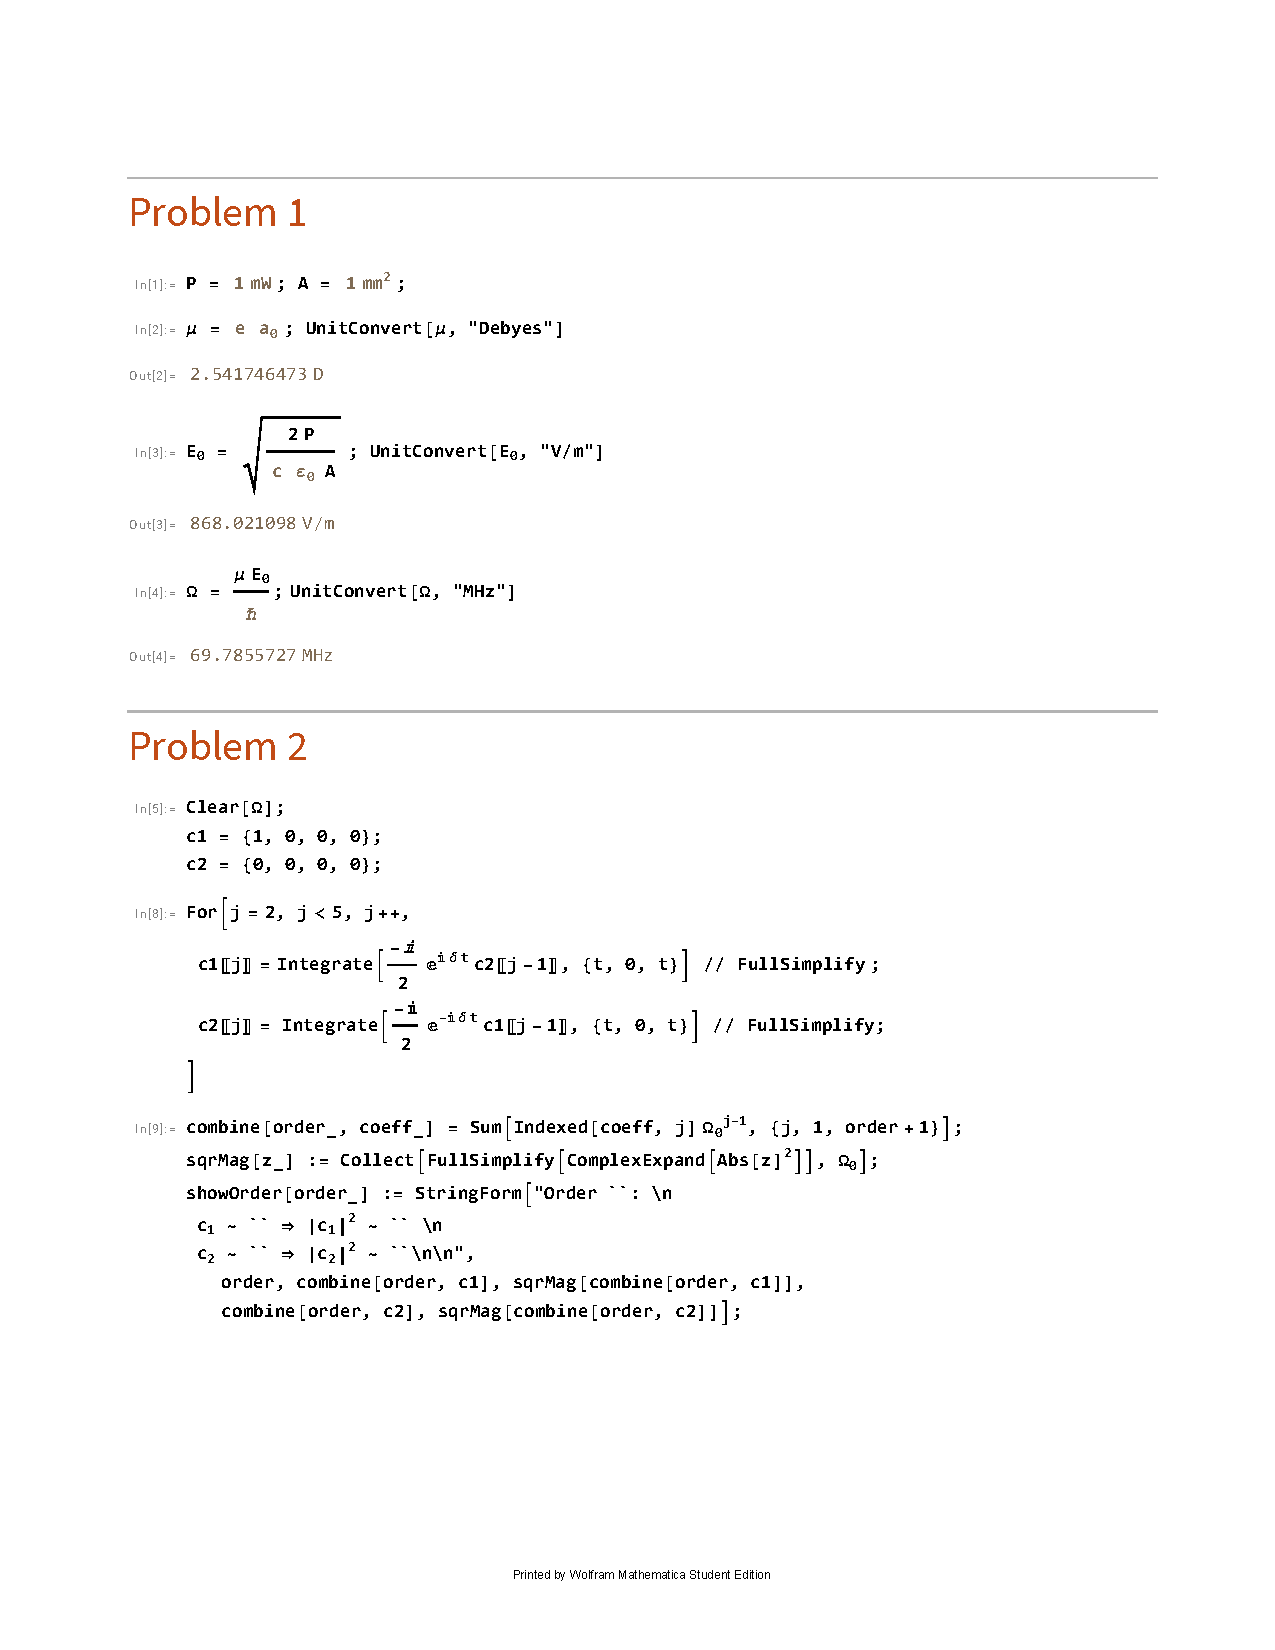
\includepdf[pages=-]{calcs/HW1_mathematica.pdf}
\end{document}